\chapter{Implementation Approach}
\label{chap:implementation}
\lhead{\emph{Implementation Approach}}
The key question to be addressed in this chapter is: "How do I plan to achieve what I have outlined in the previous chapter".
This chapter dives into the the architecture of the Docker Linter like the framework and programming languages and how they will be used to meet the functional and non-functional requirements. 

% This chapter should comprise around 5000 words and specify your planned implementation approach. Again all sections below are suggestions and will vary significantly from project to project, the key element to be addressed is the core question of the chapter.

\section{Architecture} \label{sec:Arch}
% Describe the architecture of the solution that you have in mind, including:
The architecture is designed to ensure scalability, and ease of integration.The focus is to make sure this Linter is lightweight and can be accessed on all platforms.It combines web scraping for continuous updates on the rule database, a python based linter for rule enforcement and integration with tools like Jenkins and Visual Studio Code. 
% \begin{itemize}
%     \item Technologies involved (e.g., frameworks, programming language). 
%     \item The hardware needed to develop the project (and to support at deployment stage)
% \end{itemize}
\subsection{Technologies involved}
The following framework and technologies will be used: 
\subsubsection{Programming languages}
\begin{enumerate}
    \item \textbf{Python}\\The core linter engine and the web scraper will be written in python.Python has robust libraries for text processing and supports for web scraping.\\Key libraries used: 
    \begin{itemize}
        \item \textbf{BeautifulSoup:}For web scraping to continuously fetch updates for the rules database.
        \item \textbf{json:}For structured report generation
        \item \textbf{Flask}Create an API for interacting with the linter.
    \end{itemize}
    \item \textbf{JavaScript}\\This will be used to develop the visual studio extension, as VS gives you an option between typescript and JavaScript.
\end{enumerate}
\subsubsection{Web Scraping Framework}
Web scraping refers to the automatic extraction procedure of data from websites using software. It allows us to extract data from text such as HTML, Which allows continuous updates to Dockerfile best practices are critical to ensure that the linter remains relevant.
BeautifulSoup and Requests will be the primarily used frameworks used for the web scraping.\cite{webscraping}
Web scraping involves the creation and integration of two software programs: A crawler and a scraper.
The crawler downloads data from the internet, then the scraper extracts important information in its raw form from the downloaded data and stores it in a database. \cite{webscraping}

\textbf{BeautifulSoup:}
\begin{itemize}
    \item This is a python library that allows the user to retrieve structured data from a webpage. It can be used for parsing HTML and XML, furthermore, it is much easier to use when comparing it to regular expression( a Python package) since it has fewer steps for navigating and examining a parse tree. Compared to the other tools like Regular expression or Lxml, BeautifulSoup is the slower option but suits perfectly for the linter needs a limited amount of rules. 
    \item It has the ability to automatically convert out coming document into UTF-8 and incoming document into Unicode, so the user does not need to keep track of encodings unless the document does not specify one. \cite{webscraping}
\end{itemize}
\textbf{Requests:}
\\Requests is a Python library that is used to send HTTP requests to retrieve data from the Web.It is a powerful yet easy-to-use tool that simplifies interactions with web servers, making it ideal for integration into the web scraping framework. \cite{pypy_2024}
\begin{itemize}
    \item Requests lets developers concentrate on data extraction and processing by abstracting away the hassles of sending HTTP requests, like managing sessions, cookies and headers. 
    \item Offers flexibility in communicating with different websites by supporting all major HTTP methods, like GET,POST,PUT,etc. 
    \item Provides robust and dependable web scraping by automatically addressing typical HTTP challenges like timeouts and status code failures. The lightweight performance of the linter is maintained by its efficient and lightweight design, which guarantees low latency when retrieving web pages. 
    \item Easily integrates with BeautifulSoup to parse the retrieved HTML data, resulting in a unified process for obtaining best practices. 
\end{itemize}

When collecting data from reliable sources such as, Docker's official documentation, SSL support is essential because it guarantees secure connection by supporting HTTPS right out of the box.

\textbf{Integrated Process:}
\\Requests and BeautifulSoup work together to offer a simplified method of web scrapping. 
\begin{itemize}
    \item Fetching web pages: To retrieve HTML content from dependable sources, HTTP GET requests are sent using requests. 
    \item Data Extraction and Parsing: BeautifulSoup extracts the relevant data like Docker Best Practices after parsing the HTML text. 
    \item Database storing: To keep the linter current without being dependent on a web connection, the extracted rules are processed and then saved in a local SQlite database for offline use. 
\end{itemize}

\subsubsection{Visual Studio Extension Development}
The VS Code API and a mix of web-based and IDE's specific tools are used in the development of a Visual Studio Code plugin/extension for Dockerfile linting.\\For developers, this revised method guarantees a productive, immersive and easy to use experience.\\List of tools that will be used: \\
\textbf{JavaScript:}
\begin{itemize}
    \item JavaScript is the foundation for creating VS code extensions. It is flexible and supported by a wide variety of modules accessible through npm and will be primarily used for scripting within the browsers. 
    \item It will be used for the core functionalities such as triggering linting commands and displaying results within the VS code environment. 
\end{itemize}
\textbf{Node.js:}
\\Node.js extends JavaScript's capabilities to run outside a browser environment. 
It provides access to system level features and APIs that JavaScript, in a browser, cannot access. 
\begin{itemize}
    \item \textbf{File System Access:} Reading and writing files like Dockerfiles directly from the disk. 
    \item \textbf{Process Management:}Running external programs like docker linters using modules like child process.
    \item \textbf{VS code extensions run in Node.js:} As VS code is built on Electron, which uses Node.js , extensions for VS code run in a Node.js runtime allowing developers to utilise the system level APIs
\end{itemize}

\textbf{Node Package Manager (npm):}
\\npm simplifies dependency management, ensuring extensions have access to the latest libraries and tools. 
\begin{itemize}
    \item Manages packages like Axios and XML parsers. 
    \item Streamlines the installation and updating of dependencies required for the extension's development and functionality. 
\end{itemize}

\textbf{VS Code API:}
\begin{itemize}
    \item The API provides direct access to VS Code's editor, allowing developers to  customise the UI. 
    \item Used to help Display issues in the Problems panel and highlights them directly in the Dockerfile editor.
\end{itemize} 

\textbf{Yeoman Generator:}
\begin{itemize}
    \item Yeoman scaffolds new VS Code extension projects with boilerplate code and a well-structured file system, reducing setup time.
    \item Provides a pre-configured project structure that includes necessary files like package.json, extension.js, and configuration settings.
    \end{itemize}

\subsubsection{CI/CD Integration: Jenkins}
Integration with Jenkins ensures the Docker Linter is part of the automated build and deployment pipeline.This guarantees that Dockerfiles meet quality standards before reaching production. 
\begin{itemize}
    \item Automates linter execution during build stages.
    \item Allows flexible scripting of quality checks.
\end{itemize}
Workflow: 
\begin{itemize}
    \item Dockerfiles are linted during the "Linting" stage of the pipeline.
    \item Reports are generated and archived for review.
    \item Builds fail if critical issues are detected, enforcing quality gates.
\end{itemize}

\subsection{Database : SQLite}
SQLite is chosen over MySQL for this Docker Linter Project due to its simplicity and lightweight nature.\cite{SQLite}As this project will not have multiple user access and does not needs robust security and authentication features. SQLite appears to be the better option for this project. \cite{mysql}
\\Key Functions:
\begin{itemize}
    \item Stores best practices fetched via web scraping
    \item Ensures the linter operates offline with the most recent rules.
\end{itemize}
Tables:
\begin{itemize}
    \item Columns: Rule ID, Description, Severity, Last Updated.
    \item Purpose: Stores dynamically updated best practices.
\end{itemize}
\subsubsection{Version Control: GitHub}
GitHub will host the project code, enabling collaboration and continuous integration
Key Features: 
\begin{itemize}
    \item Automates testing of the linter for quality assurance.
    \item Ensures code changes do not break existing functionality.
    \item Allows contributors to suggest enhancements and submit pull requests. %LOOK BACK OVER THIS 
    \item Tracks issues and feature requests through GitHub's Issue Tracker.
\end{itemize}

% Provide a high level view of the system you have in mind, including any package of classes, what is it responsible for and what other packages it communicates to. Provide a high level view of the database (or structure) needed to support the project, including what each table/document is responsible for and the hierarchy among them. You need to be as specific here as you can, why? Because this will aid you in identifying parts of the project you are vague on, 
% this may be fine for some components but cause problems in term 2 for others. If you have hardware element in your project this is also where you provide a high level view of how these elements integrate into the project. So for a project that is cyber-physical you will have both a hardware and software architectural diagram. N.B. This is NOT a full system design but a high level overview of what you can credibly develop. This architecture should be informed by prototyping activity. 

% Some of the implementation focused projects may describe how do you envision tackling the functional requirements of your project via a set of use-cases. DFDs are also helpful here to understand elements of your project that may cause problems. You should describe the role of the different parts of the architecture of the solution, and the interaction among them.



\section{Risk Assessment}


% Identify any potential risk precluding you from successfully complete your project. This section is really important and often neglected by students resulting in fatal risks occurring in some projects. Make sure to give this section the time it requires. Classify the risk according to their importance, possibility of arising and enumerate the decisions you can make to anticipate them or mitigate them (in case they finally arise). Table \ref{tab:ProjRisks} may help with this classification. This section should include your mitigation approach for any critical risks.

\begin{table}[h]
\centering
\scriptsize
\caption{Initial Risk Matrix for the Docker Linter Project}
\begin{tabular}{|p{2cm}|p{2cm}|p{2cm}| p{2cm} |p{2cm}| p{2cm}|}
\hline \bf Frequency/ Consequence & \bf 1-Rare & \bf 2-Remote & \bf 3-Occasional & \bf 4-Probable & \bf 5-Frequent \\ [10pt]

\hline \bf 4-Fatal & \cellcolor{yellow!50} Issues with integrating CI/CD tools like Jenkins & \cellcolor{red!50} Data loss during database updates & \cellcolor{red!50} Major bug in rule-checking algorithm & \cellcolor{red!50} Failure to meet unique feature requirements & \cellcolor{red!50} \\ [10pt]

\hline \bf 3-Critical & \cellcolor{green!50} Outdated scraped rules & \cellcolor{yellow!50}  & \cellcolor{yellow!50} Rule conflicts across sources & \cellcolor{red!50} Poor performance with large Dockerfiles & \cellcolor{red!50} Web scraper failure \\ [10pt]

\hline \bf 2-Major & \cellcolor{green!50}  & \cellcolor{green!50}  & \cellcolor{yellow!50} Missing some smells during analysis & \cellcolor{yellow!50}  & \cellcolor{red!50}  \\ [10pt]

\hline \bf 1-Minor & \cellcolor{green!50} & \cellcolor{green!50} Rare formatting issues in reports & \cellcolor{green!50}  & \cellcolor{yellow!50}  & \cellcolor{yellow!50}  \\ [10pt]
\hline
\end{tabular} \\
\label{tab:ProjRisks}
\end{table}

\subsection{Detailed Risk Assessment}
\textbf{Risk 1: Issues with Integrating CI/CD Tools Like Jenkins}
\begin{itemize}
    \item \textbf{Frequency:}Rare 
    \item \textbf{Consequences:}Fatal 
    \item \textbf{Mitigation:}Rigorous testing with Jenkins pipelines during development and creating clear integration                       documentation to ensure seamless compatibility. 
\end{itemize}
\textbf{Risk 2: Data Loss During Database Updates }
\begin{itemize}
    \item \textbf{Frequency:}Remote 
    \item \textbf{Consequences:}Fatal 
    \item \textbf{Mitigation:}Rigorous testing with Jenkins pipelines during development and creating clear integration documentation to ensure seamless compatibility. 
\end{itemize}
\textbf{Risk 3: Major Bug in the Rule Checking Algorithm }
\begin{itemize}
    \item \textbf{Frequency:}Occasional 
    \item \textbf{Consequences:}Fatal 
    \item \textbf{Mitigation:}Ensure regular unit testing and peer reviews are being implemented.
\end{itemize}
\textbf{Risk 4: Failure to Meet Unique Feature Requirements }
\begin{itemize}
    \item \textbf{Frequency:}Probable
    \item \textbf{Consequences:}Fatal 
    \item \textbf{Mitigation:}Guarantee delivery of unique features by setting a clear deadline and test the web scraper continuously. 
\end{itemize}
\textbf{Risk 5: Outdated Scraped Rules }
\begin{itemize}
    \item \textbf{Frequency:}Rare 
    \item \textbf{Consequences:}Critical 
    \item \textbf{Mitigation:}Schedule regular scraper runs and implement notifications for failures in scraping processes. 
\end{itemize}
\textbf{Risk 6:Rule Conflicts Across Sources }
\begin{itemize}
    \item \textbf{Frequency:}Occasional 
    \item \textbf{Consequences:}Critical 
    \item \textbf{Mitigation:}Add a manual validation step to ensure that rules from trusted sources align and avoid inconsistencies.
\end{itemize}
\textbf{Risk 9: Poor Performance with Large Dockerfiles}
\begin{itemize}
    \item \textbf{Frequency:}Probable
    \item \textbf{Consequences:}Critical 
    \item \textbf{Mitigation:}Optimize the rule-checking algorithm and implement caching mechanisms to improve performance.
\end{itemize}
\textbf{Risk 10: Web Scraper Failure}
\begin{itemize}
    \item \textbf{Frequency:}Frequent
    \item \textbf{Consequences:}Critical 
    \item \textbf{Mitigation:} Build robust error-handling mechanisms and regularly update the scraper to adapt to structural changes in source websites.
\end{itemize}
\textbf{Risk 11: Minor Misalignments in IDE Integration}
\begin{itemize}
    \item \textbf{Frequency:}Rare
    \item \textbf{Consequences:}Rare
    \item \textbf{Mitigation:} Conduct rigorous testing of IDE functionality and gather user feedback to resolve discrepancies.
\end{itemize}
\textbf{Risk 12: Occasional Linter Feedback Delays}
\begin{itemize}
    \item \textbf{Frequency:}Remote
    \item \textbf{Consequences:}Major
    \item \textbf{Mitigation:} Optimize the linter’s performance, particularly for real-time feedback in IDEs and CI/CD integrations.
\end{itemize}
\textbf{Risk 13: Missing Some Smells During Analysis}
\begin{itemize}
    \item \textbf{Frequency:}Occasional
    \item \textbf{Consequences:}Major
    \item \textbf{Mitigation:} Enhance the rule-checking algorithm and ensure comprehensive coverage of all relevant Docker smells.
\end{itemize}
\textbf{Risk 14: Rare Formatting Issues in Reports}
\begin{itemize}
    \item \textbf{Frequency:}Remote
    \item \textbf{Consequences:}Minor
    \item \textbf{Mitigation:} Implement robust formatting checks in the reporting module to ensure consistency.
\end{itemize}

\section{Methodology}
% Describe your personal approach on how to tackle the different parts of this project, including:
% \begin{itemize}
%     \item How to tackle the needed research to fulfil the background chapter. 
%     \item How to set up your Computer Science skills to the project needs (e.g., describe your plan to learn any new technology involved on the project that you are not familiar with). 
%     \item What core project managing approach will you follow (e.g., Waterfall, Scrum, etc).
% \end{itemize}
\subsection{Tackling Research for the Background Chapter}
To develop a strong foundation for the background chapter, I employed a systematic approach to explore relevant literature, tools, and technologies. The key steps included:

\subsubsection{Literature Review}
\begin{itemize}
    \item Analysed scholarly articles and technical reports on Docker linting tools, such as Hadolint and Snyk, to understand their functionalities and limitations.
    \item Explored empirical studies on Dockerfile smells and their impact on containerized environments, focusing on security, efficiency, and maintainability.
\end{itemize}

\subsubsection{Industry Best Practices:}
\begin{itemize}
    \item Referenced Docker's official documentation and other trusted sources to understand the latest best practices and configuration guidelines for Dockerfiles.
    \item Studied real-world case studies on DevOps workflows to identify challenges and opportunities for automation in CI/CD pipelines.
\end{itemize}
\subsubsection{Gap Analysis:}
\begin{itemize}
    \item Conducted a comparative analysis of existing Docker linting tools to identify the unique features required for the proposed linter, such as real-time feedback and dynamic rule updates.
\end{itemize}

\subsection{Aligning Computer Science Skills with Project Needs}
To meet the technical requirements of this project, I devised a plan to build upon my existing skills and acquire knowledge in new areas:

\subsubsection{Programming Languages:}
\begin{itemize}
    \item \textbf{Python:} Strengthened proficiency in Python for developing the core linter engine and web scraper. Utilized resources like online courses and documentation to gain expertise in libraries like BeautifulSoup and Flask.
    \item \textbf{JavaScript} Learned JavaScript to create the Visual Studio Code extension, focusing on utilizing the VS Code API and Node.js runtime.
\end{itemize}

\subsubsection{Web Scraping and Automation:}
\begin{itemize}
    \item Explored tutorials and documentation on BeautifulSoup and Requests to implement efficient and reliable web scraping for dynamic rule updates.
\end{itemize}

\subsubsection{CI/CD Pipeline Integration:}
\begin{itemize}
    \item Acquired knowledge in Jenkins and GitHub Actions to seamlessly integrate the linter into automated build workflows.
\end{itemize}

\subsubsection{Database Management:}
\begin{itemize}
    \item Learned SQLite for lightweight and efficient data storage of best practices and linting rules, ensuring offline functionality.
\end{itemize}

\subsubsection{Tool Familiarization:}
\begin{itemize}
    \item Conducted hands-on experiments with existing tools like Hadolint to understand their workflow and identify areas for improvement.
\end{itemize}

\subsection{Project Management Approach}
To ensure structured development and timely delivery, I opted for an Agile-Scrum methodology:

\subsubsection{Sprint Planning:}
\begin{itemize}
    \item Divided the project into manageable sprints, each with clearly defined goals, such as developing the core linter engine, implementing web scraping, and integrating CI/CD functionality.
\end{itemize}

\subsubsection{Daily Stand ups:}
\begin{itemize}
    \item Used daily stand-ups to track progress and identify blockers, ensuring constant alignment with project objectives.
\end{itemize}

\subsubsection{Iterative Development:}
\begin{itemize}
    \item Adopted an iterative approach, refining features based on feedback and testing at the end of each sprint.
\end{itemize}
\subsubsection{Tools for Collaboration:}
\begin{itemize}
    \item GitHub was used for version control and issue tracking, ensuring efficient collaboration and code quality.
\end{itemize}

\subsubsection{Risk Management:}
\begin{itemize}
    \item Periodically revisited the risk assessment matrix to proactively address challenges, such as outdated scraped rules or integration issues.
\end{itemize}

This methodology not only ensures a comprehensive and adaptive approach to project execution but also aligns with industry standards for software development and DevOps practices.

\section{Implementation Plan Schedule}
% Come up with a schedule for the remaining time (including second semester), so as to describe how do you envision to achieve the implementation of your project by the end of semester 2. This plan SHOULD be ambitious but MUST be realistic and SHOULD be informed by early prototyping and MUST be discussed with your term 1 supervisor.
\subsection{Semester 1 (Research Phase)}
\textbf{Goal:} Complete foundational research, define requirements, and prototype key components.
\textbf{December - January} 
\begin{enumerate}
    \item Prototype development
    \begin{itemize}
        \item Create architectural diagrams and define the system architecture of the Docker Linter.
        \item Develop a basic prototype for Dockerfile analysis focusing on rule enforcement for critical "Docker smells," such as unpinned dependencies and redundant layers.
        \item Test and validate the prototype against sample Dockerfiles to ensure functionality.
    \end{itemize}
    \item Presentation and Feedback
    \begin{itemize}
        \item Present initial findings and the prototype to your supervisor for refinement and approval of the implementation plan.
    \end{itemize}
\end{enumerate}

\subsection{Semester 2 (Implementation Phase)}
\textbf{Goal:} Develop, test, and validate the Docker Linter.

\textbf{January (Kick-off)} 
\begin{enumerate}
    \item Implementation Setup
    \begin{itemize}
        \item Finalize tools and technologies (e.g., SQLite for local rules storage, Flask for API).
        \item Set up development environment (e.g., GitHub for version control, Jenkins for CI/CD integration).
    \end{itemize}
    \item Enhance Prototype
    \begin{itemize}
        \item Extend the web scraper to fetch a comprehensive rule database.
        \item Implement Dockerfile analysis logic for a broader set of "smells."
    \end{itemize}
\end{enumerate}

\textbf{February}
\begin{enumerate}
    \item IDE Integration (Visual Studio Code)
    \begin{itemize}
        \item Develop a VS Code extension for real-time feedback on Dockerfiles.
        \item Test UI/UX for user-friendly error highlighting and suggestions.
    \end{itemize}
    \item Database Integration
    \begin{itemize}
        \item Use SQLite for rule storage with support for offline analysis.
        \item Enable dynamic updates using the web scraper.
    \end{itemize}
\end{enumerate}

\textbf{March}
\begin{enumerate}
    \item CI/CD Integration
    \begin{itemize}
        \item Integrate the linter with Jenkins and GitHub Actions to automate quality checks.
        \item Develop pipelines to test Dockerfiles during build stages.
    \end{itemize}
    \item Performance Optimization
    \begin{itemize}
        \item Optimize rule-checking algorithms for speed with large Dockerfiles.
        \item Implement caching mechanisms for reused Dockerfiles.
    \end{itemize}
\end{enumerate}

\textbf{April}
\begin{enumerate}
    \item Testing and Validation
    \begin{itemize}
        \item Test on real-world Dockerfiles to validate the accuracy of "smell" detection.
        \item Conduct unit testing for core features and load testing for large-scale usage.
    \end{itemize}
    \item Generate Quality Reports
    \begin{itemize}
        \item Develop report templates for CI/CD pipelines and standalone analyses.
        \item Include severity-based prioritization of issues.
    \end{itemize}
\end{enumerate}

\textbf{May}
\begin{enumerate}
    \item Documentation
    \begin{itemize}
        \item Write detailed user documentation for installation and usage.
        \item Prepare technical documentation for the codebase.
    \end{itemize}
    \item Final Adjustments
    \begin{itemize}
        \item Incorporate feedback from beta testing.
        \item Polish UI and resolve any outstanding issues.
    \end{itemize}
\end{enumerate}

\textbf{June}
\begin{enumerate}
    \item Project Submission and Presentation
    \begin{itemize}
        \item Submit the completed Docker Linter project with comprehensive documentation and demo.
        \item Present findings and showcase the tool's functionality to your supervisor and peers.
    \end{itemize}
\end{enumerate}

\section{Evaluation}
% Come up with an evaluation plan that allows you to measure how much have you actually achieved the goals of your project. This again is a section that is often neglected where students loose marks. How do you plan to measure the output of your project? A binary it works/does not work is insufficient. You need to be able to quantify the success against both the functional requirements and the initial idea. These are not the same as you may meet all function requirements outlined but not solve the overall problem because you have failed to revisit these and update them with new information which you learn as you are developing the project.
\subsection{Objectives Alignment}
Define metrics for each project goal to measure whether they are met effectively.

\subsubsection*{Functional Goals}
\begin{itemize}
    \item \textbf{Real-Time Dockerfile Analysis}
    \begin{itemize}
        \item Average latency (in milliseconds) for feedback after edits.
        \item Precision and recall of detected "Docker smells."
    \end{itemize}

    \item \textbf{Smell Detection and Categorization}
    \begin{itemize}
        \item Number of predefined "Docker smells" accurately detected during a controlled test with various Dockerfiles.
        \item User feedback on clarity of categorization (collected via surveys or interviews).
    \end{itemize}

    \item \textbf{IDE Integration}
    \begin{itemize}
        \item Developer satisfaction (survey results or Net Promoter Score) using the IDE plugin.
        \item Percentage of identified issues resolved directly in IDEs.
    \end{itemize}

    \item \textbf{CI/CD Pipeline Compatibility}
    \begin{itemize}
        \item Successful integration rate in CI/CD environments (e.g., Jenkins, GitHub Actions).
        \item Detection and prevention rate of invalid Dockerfiles in CI/CD pipelines.
    \end{itemize}
\end{itemize}

\subsubsection{Project Goals}
\begin{itemize}
    \item \textbf{Enhancing Security}
    \begin{itemize}
        \item Number of security issues flagged and resolved per Dockerfile compared to baseline tools (e.g., Hadolint, Snyk).
        \item Reduction in incidents of deploying vulnerable images after using the linter.
    \end{itemize}

    \item \textbf{Optimizing Performance}
    \begin{itemize}
        \item Average image size and build time improvement after applying linter recommendations.
        \item Rate of compliance with optimization rules (e.g., multi-stage builds, minimized layers).
    \end{itemize}

    \item \textbf{Developer Productivity}
    \begin{itemize}
        \item Time saved per Dockerfile review compared to manual methods.
        \item Survey results on perceived efficiency gains after adoption.
    \end{itemize}
\end{itemize}

\subsection{Evaluation Methods}
\subsubsection{Quantitative Metrics}
\begin{itemize}
    \item \textbf{Automated Testing}: Use predefined Dockerfiles with known issues to test detection accuracy and recommendation validity.
    \item \textbf{Performance Logging}: Log the linter's processing times, detected issues, and resolution effectiveness in real scenarios.
\end{itemize}

\subsubsection{Qualitative Metrics}
\begin{itemize}
    \item \textbf{Developer Surveys}: Conduct pre- and post-implementation surveys with questions on usability, clarity, and efficiency improvements.
    \item \textbf{Feedback Loops}: Gather anecdotal feedback from developers and DevOps engineers on workflow integration.
\end{itemize}

\subsection{Controlled Experiments}
\begin{itemize}
    \item Develop a benchmark dataset of Dockerfiles with annotated issues.
    \item Compare the linter's performance against existing tools like Hadolint and Snyk for:
    \begin{itemize}
        \item Detection accuracy.
        \item Remediation prioritization.
        \item Efficiency improvements (image size, build time).
    \end{itemize}
\end{itemize}

\subsection{Real-World Testing}
\subsubsection{Pilot Deployment}
Integrate the linter in a live CI/CD pipeline for a selected team/project and measure the following:
\begin{itemize}
    \item Incident rate reduction.
    \item Time to resolve flagged issues.
\end{itemize}

\subsubsection{Long-Term Monitoring}
Track Dockerfile quality over a defined period and compare it with historical data.

\subsection{Reporting and Documentation}
\begin{itemize}
    \item Generate reports summarizing findings for each metric.
    \item Include visual data representation (charts/graphs) for clarity.
    \item Provide actionable insights and areas for future improvement based on results.
\end{itemize}

\section{Prototype}
% Although you do not have a fully functional project yet, you should show wireframes, snapshots or representation on how do you envision your project to look once the implementation phase has been completed. The nature of this section will vary significantly from project to project and can include anything from code snippets to snapshots of service deployments. Any prototyping you have done during the term should be summarized here that has not been captured in earlier sections. For example if you are planning to host your project using AWS in an EC2 instance you should have at least created a "hello world" setup to determine the basics, this probably should have been discussed in section \ref{sec:Arch}.
\begin{figure}
    \centering
    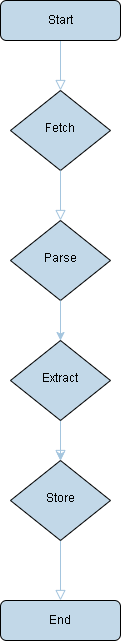
\includegraphics[height=15cm]{Figures/Web Scraper FlowChart.png} % Adjust the height here
    \caption{Web Scraper Flow Chart}
    \label{fig:enter-label}
\end{figure}


\begin{figure}
    \centering
    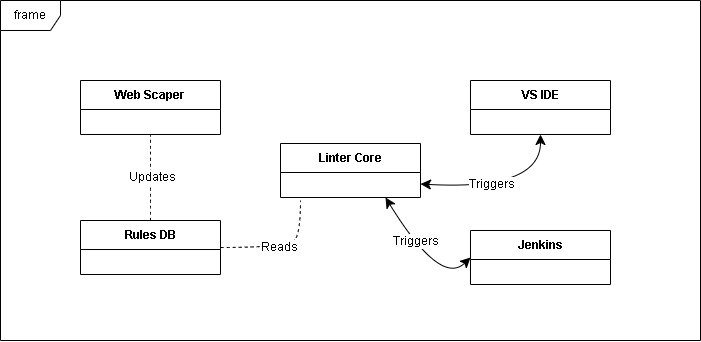
\includegraphics[width=1\linewidth]{Figures/UML.png}
    \caption{High level Overview}
    \label{fig:enter-label}
\end{figure}

\begin{figure}
    \centering
    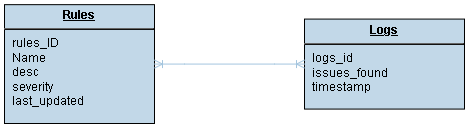
\includegraphics[width=1\linewidth]{Figures/database.drawio.png}
    \caption{Database Schema}
    \label{fig:enter-label}
\end{figure}
\begin{figure}
    \centering
    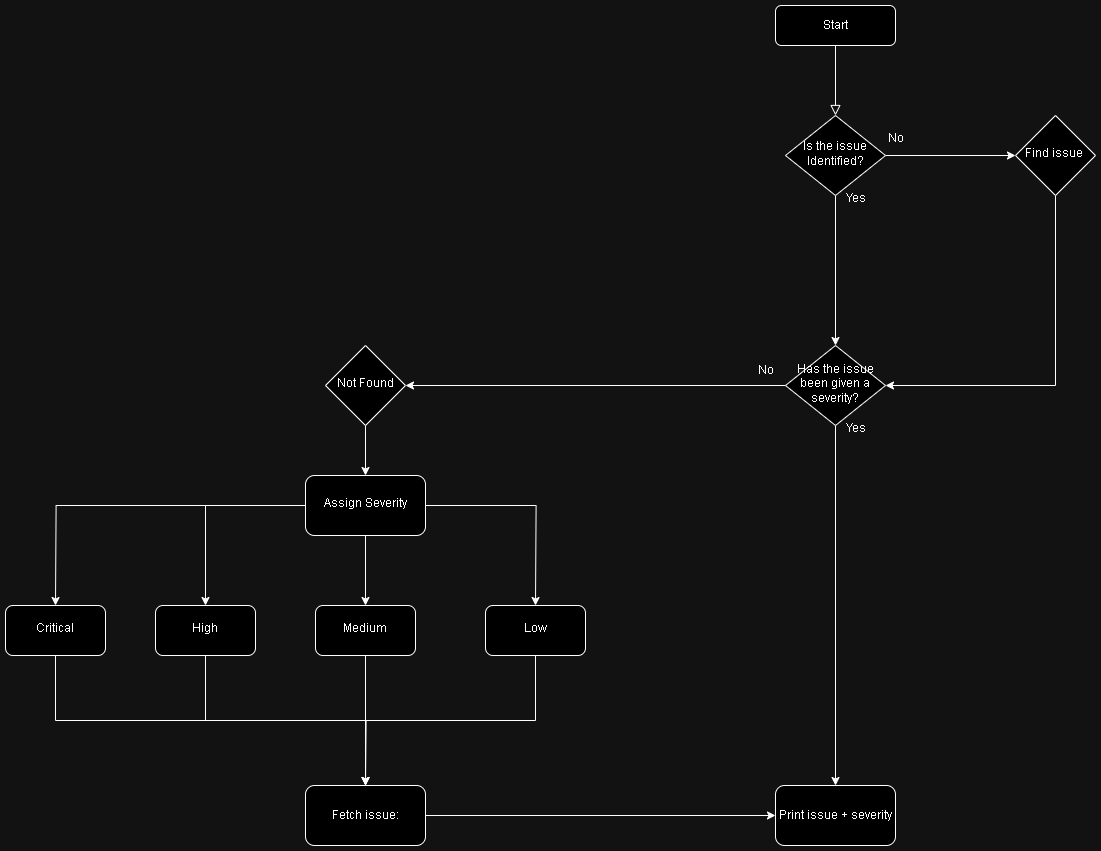
\includegraphics[width=1\linewidth]{Figures/prioritisation.drawio.png}
    \caption{Prioritisation Flow Chart}
    \label{fig:enter-label}
\end{figure}